\section{Metodo \textit{Equals()}}
L’operatore binario == viene utilizzato per stabilire se il contenuto di due variabili è identico. Per i tipi non primitivi viene confrontato il contenuto dei puntatori degli oggetti, ovvero l’indirizzo di memoria degli oggetti a cui i puntatori fanno riferimento.
Spesso però potremmo avere oggetti che nonostante puntino ad indirizzi di memoria differenti possono essere considerati a tutti gli effetti uguali.
La procedura standard per confrontare oggetti in Java è il metodo\textbf{equals()}, definito in \textbf{Object}, quindi è disponibile su tutti gli oggetti (ma non sui tipi primitivi):
\begin{lstlisting}
/*segnatura*/
public boolean equals(Object x)

/*implementazione*/
public boolean equals(Object obj) {
  return this == obj;
}

\end{lstlisting}
Il confronto viene fatto con l’operatore ==, dato che non è possibile conoscere in Object come confrontare qualsiasi oggetto Java.  Per effettuare un confronto migliore non basato sugli indirizzi di memoria, è buona norma effettuare l’overriding del metodo equals in ogni classe che sviluppiamo.

\subsection{Proprietà del metodo \textit{Equals()}}
Il linguaggio Java richiede che qualunque ridefinizione del metodo equals() rispetti determinate proprietà che forniscono una vera e propria \textbf{relazione di equivalenza}:
\begin{itemize}
\item \textbf{Riflessività}; per ogni oggetto x, avremo che x.equals(x) ritorna \textit{true};
\item \textbf{Simmetria}: dati due oggetti x ed y, avremo che se x.equals(y) ritorna true, allora y.equals(x) ritorna \textit{true};
\item \textbf{Transitività}: dati tre oggetti x, y e z, se x.equals(y) ritorna true e y.equals(z) ritorna true, allora x.equals(z) ritorna \textit{true}.
\end{itemize}

\subsection{Corretta implementazione di \textit{Equals()}}
Si devono eseguire 3 step nella classe più un quarto di verifica all'esterno:
\begin{enumerate}
\item Usare == per vedere se l'argomento è uguale a this;
\begin{lstlisting}
if(this == obj) return true;
\end{lstlisting}

\item Verificare se l’oggetto passato al metodo è del tipo desiderato, effettuando un controllo con l’operatore \textit{instanceof}, in caso negativo restituiremo false;
\begin{lstlisting}
if(!(obj istanceof ClassName)) return false;
\end{lstlisting}

\item Essendo sicuri di avere un oggetto del tipo desiderato, potremo effettuare in sicurezza un downcast al tipo desiderato. In questo modo possiamo accedere ai campi e metodi prima nascosti a causa del riferimento di tipo Object utilizzato;
\begin{lstlisting}
NomeClasse cp = (NomeClasse)ogj;
return cp.campo1.equals(this.campo1) &&
 cp.campoN.equals(this.campoN);
\end{lstlisting}

\item Confrontare se stiamo rispettando la riflessibilità, simmetria e transitività.
\end{enumerate}

\begin{figure}[H]
\centering
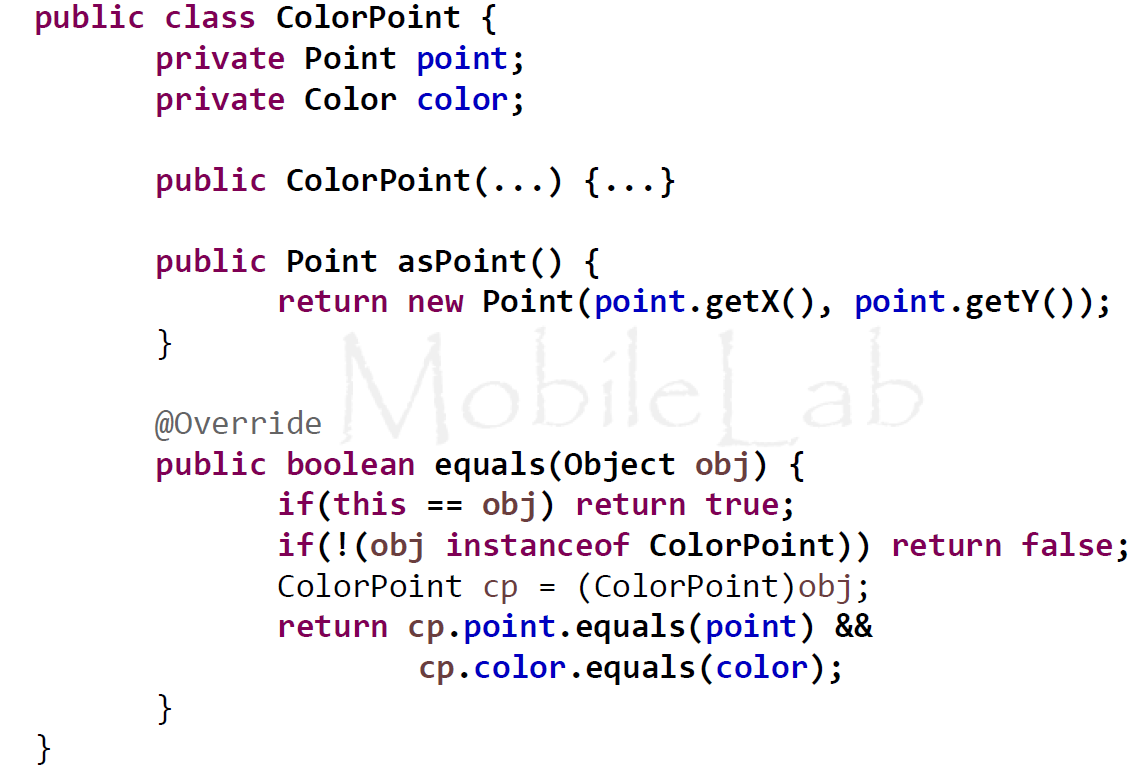
\includegraphics[scale=0.42]{images/imgEquals}
\caption{Implementazione corretta di equals\label{fig:UC3}}
\end{figure}

\subsection{Binding dinamico di \textit{Equals()}}
Quando si effettua l’overriding di equals, è sconsigliato cambiare il tipo del parametro di equals Object , altrimenti non avremo un overriding ma un overloading. Questo cambiamento potrebbe provocare disastri, vediamo con un esempio in cui cambiando il tipo del parametro di equals cosa potrebbe accadere:
\begin{lstlisting}
public boolean equals(Employee e){}
\end{lstlisting}
Inoltre supponeremo di avere:
\begin{lstlisting}
	Emplyee e1 = new Employee(...);
  	Emplyee e2 = new Employee(...);
  	Object o1 = e1;
  	Object o2= e1;
\end{lstlisting}
 Analizziamo cosa succede ad ogni riga con l’utilizzo del Binding dinamico:
\begin{itemize}
\item \textbf{o1.equals(o2);} Le firme candidate sono cercate solo in Object perché il tipo dichiarato di o1 è Object. Di conseguenza non verrà considerata la specializzazione del metodo equals effettuata;
\item \textbf{o1.equals(e2);} Nella fase 2 del Binding dinamico non c’è overriding , quindi verrà preso l’unico metodo equals esattamente uguale che sarà quello contenuto in Object. Anche in questo caso non verrà considerata la specializzazione del metodo equals che abbiamo effettuato;
\item \textbf{e1.equals(o1);} Viene valutato ma Object non è assegnabile a Employee. Di conseguenza non verrà considerata la specializzazione del metodo equals effettuata;
\item \textbf{e1.equals(e2);} La firma combacia con quella specializzata e sarà l’unico caso in cui verrà chiamato il “giusto” equals.
\end{itemize}

\subsection{Metodo \textit{Equals()} ed eredità}
Quando il metodo equals viene sovrascritto bisogna prestare attenzione al funzionamento tra il metodo equals definito e il suo funzionamento nelle classi sottostanti. In definitiva bisogna decidere come si deve comportare il metodo equals con le sue sottoclassi. In particolare, bisogna porsi due domande:

\begin{enumerate}
\item \textbf{Il criterio di confronto tra oggetti di una sottoclasse è diverso da quello che vale tra oggetti della superclasse?}
\begin{itemize}
\item No, allora bisogna definire equals della superclasse final in modo che nessuna sottoclasse possa sovrascriverlo;
\item Si, allora il metodo equals deve essere opportunamente ridefinito in ogni sottoclasse in cui il criterio di confronto è differente.
\end{itemize}
\item \textbf{Un oggetto di una sottoclasse può essere considerato uguale ad un oggetto di una superclasse?}
\begin{itemize}
\item No, allora bisogna verificare di ammettere il confronto solo tra agli oggetti del tipo giusto;
\item Si, allora se gli oggetti di una sottoclasse possono essere considerati uguali a quelli di una superclasse dovremo ammettere al confronto tutti gli oggetti di quel tipo e tutte le sue sottoclassi.
\end{itemize}
\end{enumerate}

\subsection{Tipi primitivi vs oggetti}
Si sente dire spesso l’affermazione \textit{in Java tutto è un oggetto}. In realtà questa frase non è del tutto vera in quanto esistono i tipi primitivi che permettono di utilizzare numeri, caratteri e valori booleani senza ricorrere agli oggetti. I tipi primitivi sono riconoscibili anche perché iniziano con una lettera minuscola (mentre i nomi delle classi iniziano sempre con una maiuscola). I tipi primitivi disponibili in Java sono i seguenti:
\begin{itemize}
\item \textbf{boolean:} valore booleano, può assumere i valori true e false;
\item \textbf{byte:} numero intero a 8 bit;
\item \textbf{short:} numero intero a 16 bit;
\item \textbf{int:} numero intero a 32 bit;
\item \textbf{long:} numero intero a 64 bit;
\item \textbf{float:} numero reale a 32 bit in virgola mobile (IEEE 754-1985);
\item \textbf{double:} numero reale a 64 bit in virgola mobile (IEEE 754-1985);
\item \textbf{char:} carattere unicode a 16 bit;
\end{itemize}
Gli oggetti in Java sono istanze di una classe.
Una delle differenze importanti fra tipi primitivi e oggetti si ha se guardiamo la situazione della memoria a basso livello. Infatti nella locazione di memoria corrispondente a un tipo primitivo è presente il valore mentre in quella di un oggetto è presente il puntatore all’area di memoria che contiene l’oggetto. Un diagramma spiega meglio questa differenza:
\begin{lstlisting}
int i1 = 5;
int i2 = 7;
Persona p1 = new Persona("Mario", "Rossi");
Persona p2 = new Persona("Mario", "Verdi");
\end{lstlisting}
\begin{figure}[H]
\centering
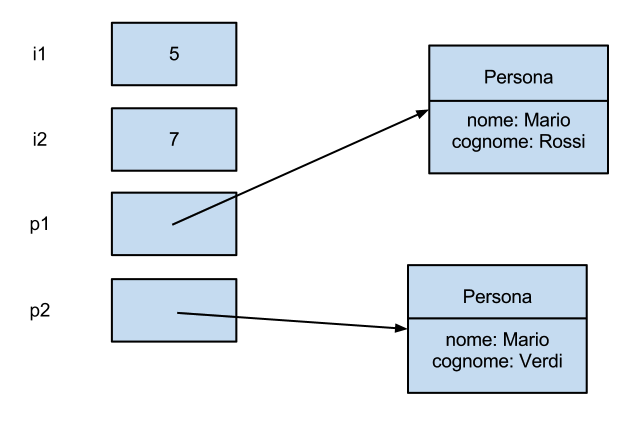
\includegraphics[scale=0.42]{images/tipiPrimitivi}
\caption{tipi primitivi e oggetti: rappresentazione in memoria\label{fig:UC3}}
\end{figure}
Fin qui sembra tutto semplice, andiamo avanti facendo un po’ di assegnazioni:
\begin{lstlisting}
i2 = i1;
p2 = p1;
\end{lstlisting}
A questo punto quale è la situazione? Ovviamente i1 e i2 assumo lo stesso valore, stessa cosa anche per p1 e p2. Ma se andiamo a vedere cosa è successo in memoria la situazione è un po’ più complicata: 	
\begin{figure}[H]
\centering
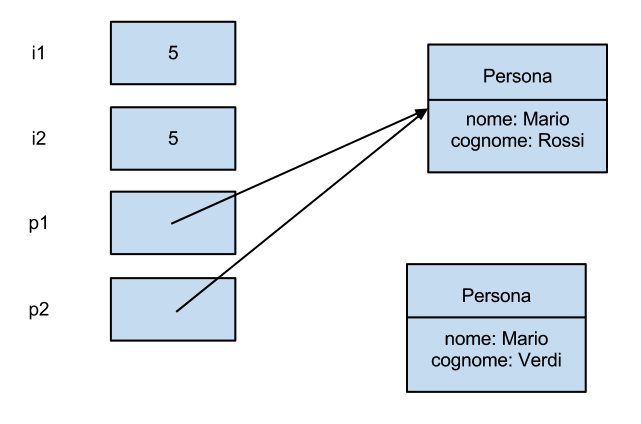
\includegraphics[scale=0.42]{images/memoria1}
\caption{tipi primitivi e oggetti: rappresentazione in memoria dopo assegnazione\label{fig:UC3}}
\end{figure}
Adesso p1 e p2 puntano allo stesso oggetto: abbiamo una condivisione di memoria che può risultare pericolosa se non gestita adeguatamente. Infatti richiamando un metodo setter su uno dei due oggetti (per esempio p1.setNome("Fabio")) si modificherà l’oggetto condiviso dai due puntatori. 

\subsection{\textit{Equals()} Vs ==}
Iniziamo con l’operatore ==: invocando questo costrutto viene confrontato il valore contenuto nella variabile. Quindi, nel caso di tipi primitivi viene confrontato il valore vero, mentre nel caso di oggetti viene confrontato l’indirizzo di memoria a cui i puntatori fanno riferimento.
Vediamo un esempio concreto. Il seguente codice stampa sulla console 4 volte il valore true:
\begin{lstlisting}
int i1 = 5;
int i2 = 7;
 
System.out.println(i1 != i2);
i2 = i1;
System.out.println(i1 == i2);
 
Persona p1 = new Persona("Mario", "Rossi");
Persona p2 = new Persona("Mario", "Verdi");
 
System.out.println(p1 != p2);
p2 = p1;
System.out.println(p1 == p2);
\end{lstlisting}
p1 e p2 puntano allo stesso oggetto e quindi confrontando l’indirizzo di memoria corrispondente al puntatore si ha un esito positivo.
Vediamo un altro esempio leggermente più complicato. Definiamo due volte lo stesso valore/oggetto e confrontiamolo con ==:
\begin{lstlisting}
int i1 = 5;
int i2 = 5;
 
System.out.println(i1 == i2);
 
Persona p1 = new Persona("Mario", "Rossi");
Persona p2 = new Persona("Mario", "Rossi");
 
System.out.println(p1 == p2);
\end{lstlisting}
In questo caso la prima condizione sui tipi primitivi è vera mentre quella sugli oggetti è falsa! Il motivo è chiaro, le variabili p1 e p2 in questo caso puntano a locazioni di memoria diverse quindi confrontando gli indirizzi di memoria si avrà un risultato negativo. Per ovviare a questo problema è necessario usare il metodo equals che, a differenza dell’operatore ==, confronta gli oggetti puntati entrando quindi in merito al contenuto dell’oggetto.
Riproviamo quindi a eseguire lo stesso codice usando il metodo equals per confrontare i due oggetti:
\begin{lstlisting}
Persona p1 = new Persona("Mario", "Rossi");
Persona p2 = new Persona("Mario", "Rossi");
 
System.out.println(p1.equals(p2));	
\end{lstlisting}
Eseguendo questo codice viene stampato sulla console ancora false! Come mai? Il motivo è che il metodo equals è definito dentro la classe Object con la seguente implementazione:
\begin{lstlisting}
public boolean equals(Object obj) {
  return this == obj;
}
\end{lstlisting}
L’implementazione di Object del metodo equals utilizza l’operatore ==! Questa scelta può sembrare strana ma è l’unica che poteva essere fatta. infatti la classe Object è la classe padre di tutte le classi Java, non è possibile dentro questa classe sapere come confrontare qualunque oggetto Java! 

